\subsection{Esercizio 20}
Costruire una function, $spline0.m$, avente la \underline{stessa sintassi} della function $spline$
di Matlab, che implementi la spline cubica naturale interpolante una funzione.
\newline \textbf{Soluzione:} \newline
% \lstinputlisting{./capitolo4/minimiquadrati.m}
% Eseguendo \nameref{cod:20} si ottiene:

% 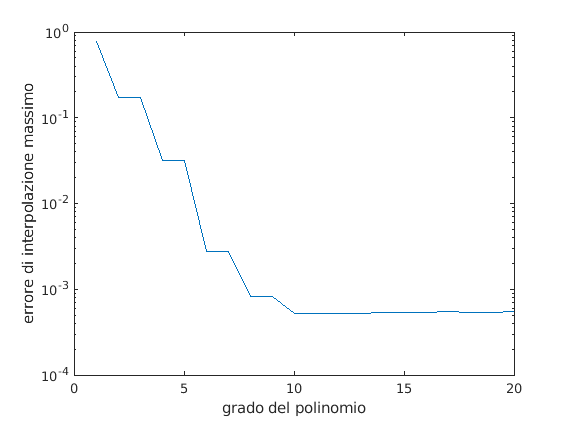
\includegraphics[scale=0.8]{capitolo4/squares.png}


% Si nota una decrescita  delll'errore  esponenziale fino a  $m = 10$, dove si assesta tra $10^{-3}$ e $10^{-4}$.